\documentclass[xcolor=x11names,compress,professionalfonts]{beamer}

%% General packages %%%%%%%%%%%%%%%%%%%%%%%%%%%%%%%%%%
\usepackage[utf8]{inputenc}
\usepackage{graphicx}
\usepackage{tikz}
\tikzset{% change default arrow tips
    >=latex
}
\usepackage{ifthen}

\usepackage{amsmath}
\usepackage{nicefrac}

%%%%%%%%%%%%%%%%%%%%%%%%%%%%%%%%%%%%%%%%%%%%%%%%%%%%%%


%% Beamer Layout %%%%%%%%%%%%%%%%%%%%%%%%%%%%%%%%%%
\useoutertheme[subsection=false,shadow]{miniframes}
\useinnertheme{rectangles}

\setbeamertemplate{navigation symbols}{}%remove navigation symbols

\usepackage{libertine}
\usepackage[T1]{fontenc}

\setbeamerfont{title like}{shape=\scshape}
\setbeamerfont{frametitle}{shape=\scshape}

\setbeamercolor*{lower separation line head}{bg=DeepSkyBlue4} 
\setbeamercolor*{normal text}{fg=black,bg=white} 
\setbeamercolor*{alerted text}{fg=red} 
\setbeamercolor*{example text}{fg=black} 
\setbeamercolor*{structure}{fg=black} 
 
\setbeamercolor*{palette tertiary}{fg=black,bg=black!10} 
\setbeamercolor*{palette quaternary}{fg=black,bg=black!10} 

\renewcommand{\(}{\begin{columns}}
\renewcommand{\)}{\end{columns}}
\newcommand{\<}[1]{\begin{column}{#1}}
\renewcommand{\>}{\end{column}}
%%%%%%%%%%%%%%%%%%%%%%%%%%%%%%%%%%%%%%%%%%%%%%%%%%

\usepackage{braket}

%%%My Math

\newcommand{\pd}[2]{\frac{\displaystyle \partial #1}{\displaystyle\partial #2}} % for partial derivatives
\newcommand{\dx}{\mathrm{d}x}
\renewcommand{\d}[1]{\mathrm{d}#1}
\newcommand{\nth}{$n^\text{th}$ }

\newcommand{\mean}[1]{\langle #1 \rangle}
\DeclareMathOperator{\Pf}{Pf}
\DeclareMathOperator{\Tr}{Tr}

\begin{document}


\begin{frame}
\title{Fractals and physics}
%\subtitle{SUBTITLE}
\author{ Nicolas Macé (inspired by E. Akkermans) }
\date{
	June 2, 2015
}
\titlepage
\end{frame}


\begin{frame}{Outline}
    \tableofcontents[hideallsubsections]
\end{frame}

\section{Fractals and their geometry}
%Each section needs a subsection for the small points on top to show up
\subsection{Dummy}

\begin{frame}{Symmetry}
    \begin{itemize}
        \item Euclidean space (continuous translational symmetry \& continuous scaling symmetry)
            \begin{itemize}
                \item Crystallographic lattice (discrete translational symmetry)
                \item Fractal set/manifold (discrete scaling symmetry)
            \end{itemize}
    \end{itemize}
    
    $\rightarrow$ fractal: infinitely divisible object
    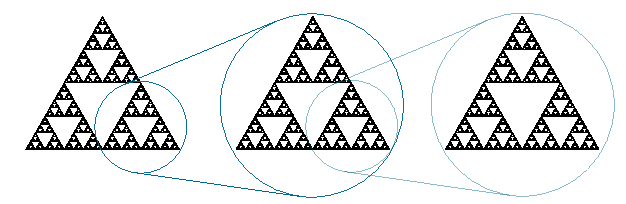
\includegraphics[scale=1.00]{sierpinski.pdf}
\end{frame}

\begin{frame}{Geometric construction}{Recursive transformations: Iterated function systems}

\begin{columns}
\newcommand{\s}{.2}
  \begin{column}{3cm}
    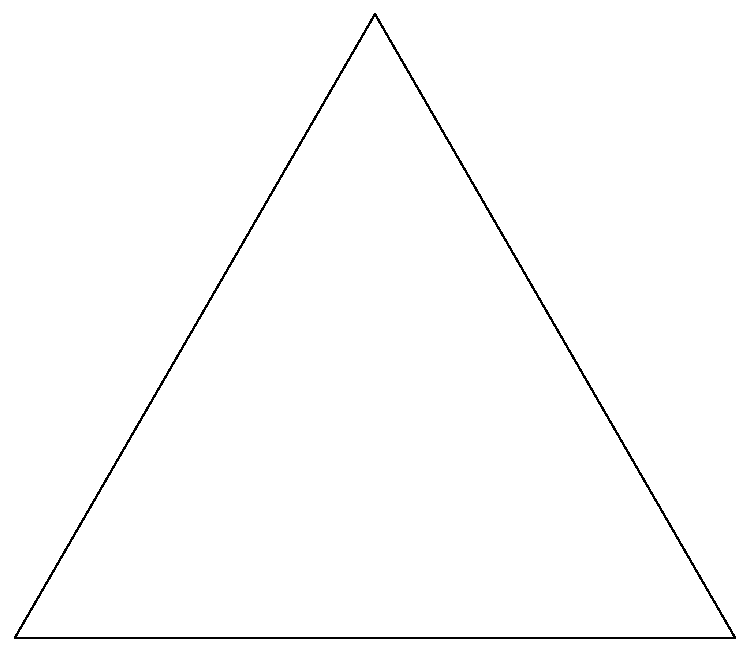
\includegraphics[scale=\s]{sierpinski0.pdf}
  \end{column}

  \begin{column}{3cm}
     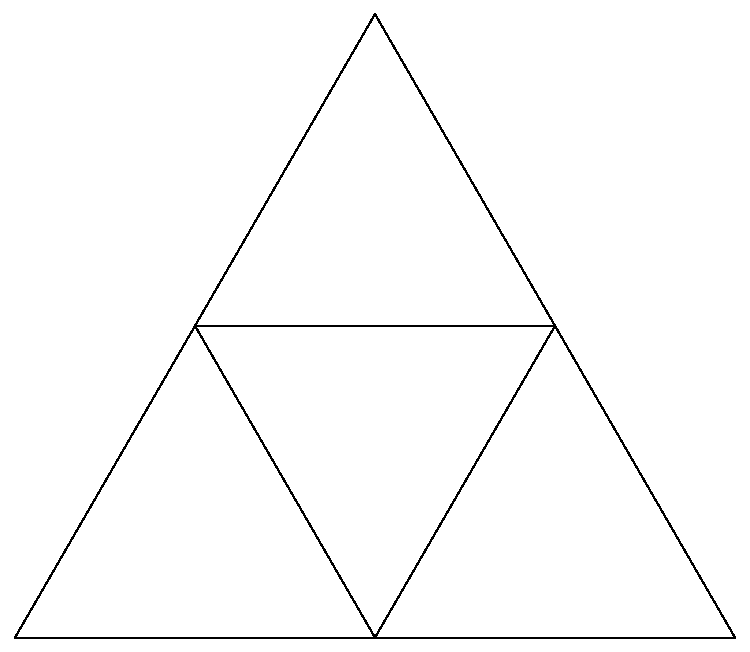
\includegraphics[scale=\s]{sierpinski1.pdf}
  \end{column}
  
  \begin{column}{3cm}
    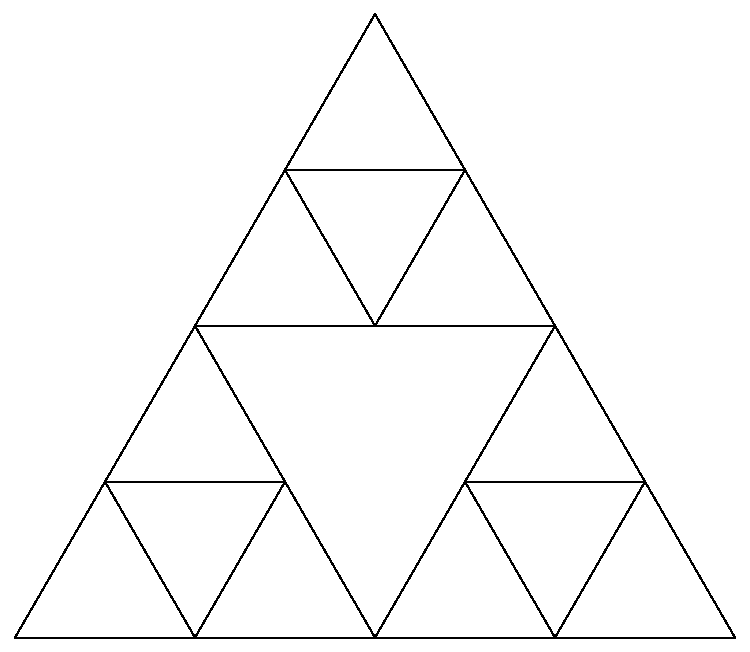
\includegraphics[scale=\s]{sierpinski2.pdf}
  \end{column}
  ...
    \begin{column}{3cm}
    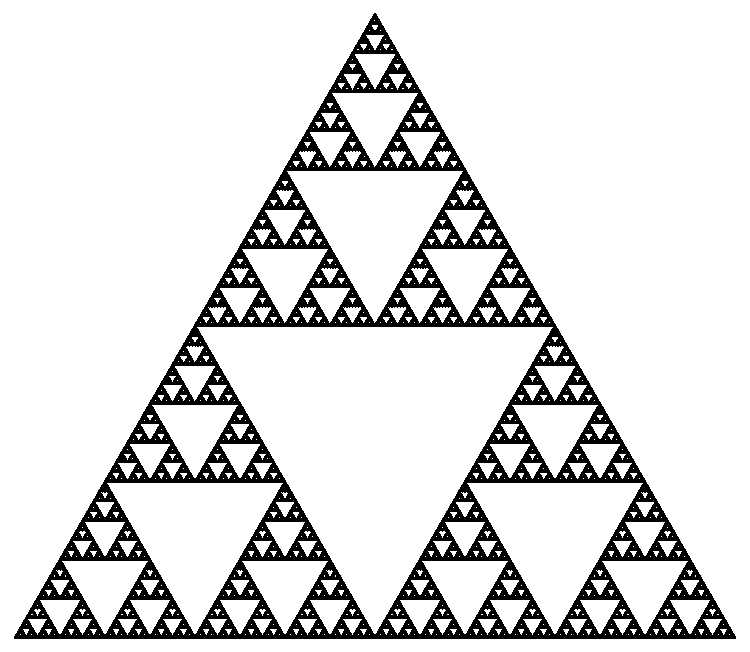
\includegraphics[scale=\s]{sierpinskiInfty.pdf}
  \end{column}
\end{columns}

~

\begin{columns}
\newcommand{\s}{.2}
  \begin{column}{3cm}
    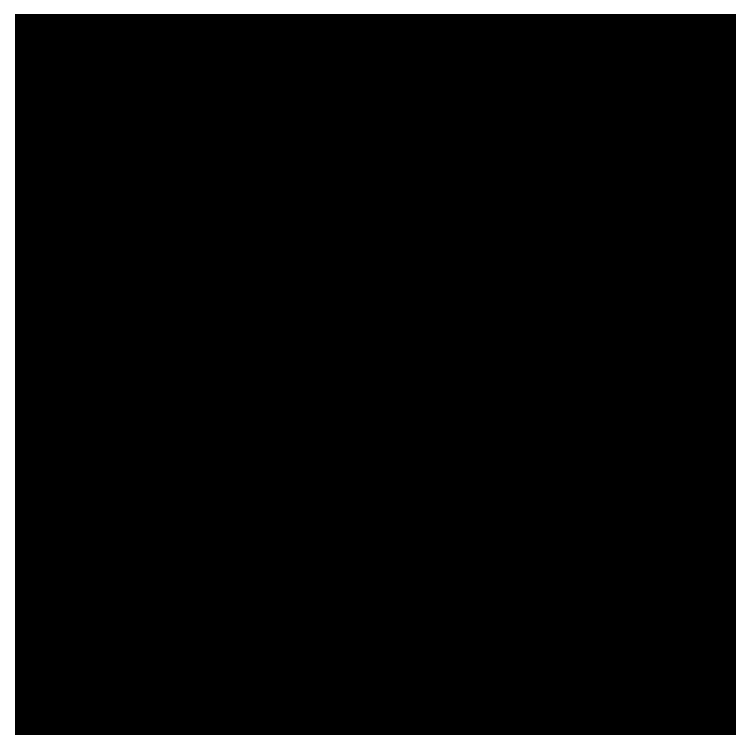
\includegraphics[scale=\s]{leaf0.pdf}
  \end{column}

  \begin{column}{3cm}
     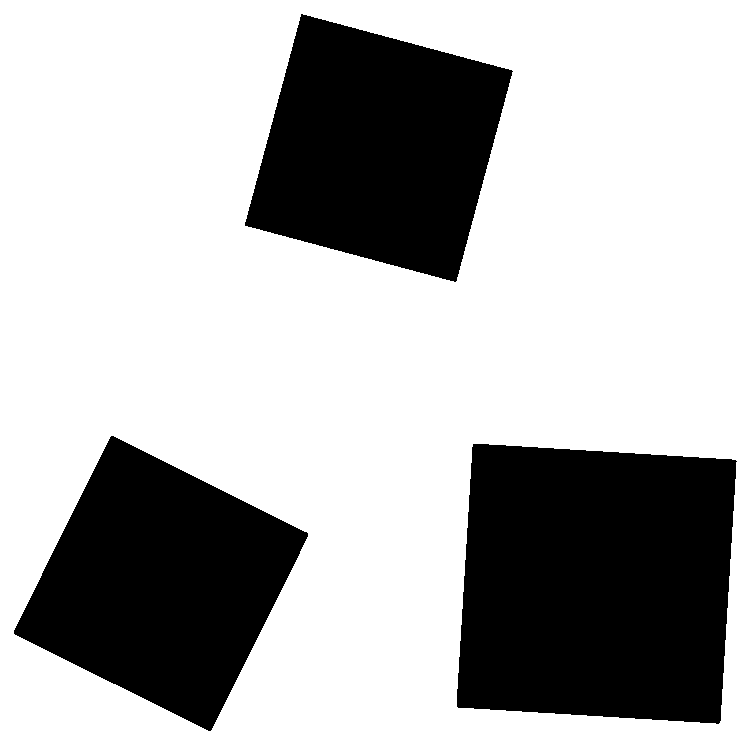
\includegraphics[scale=\s]{leaf1.pdf}
  \end{column}
  
  \begin{column}{3cm}
    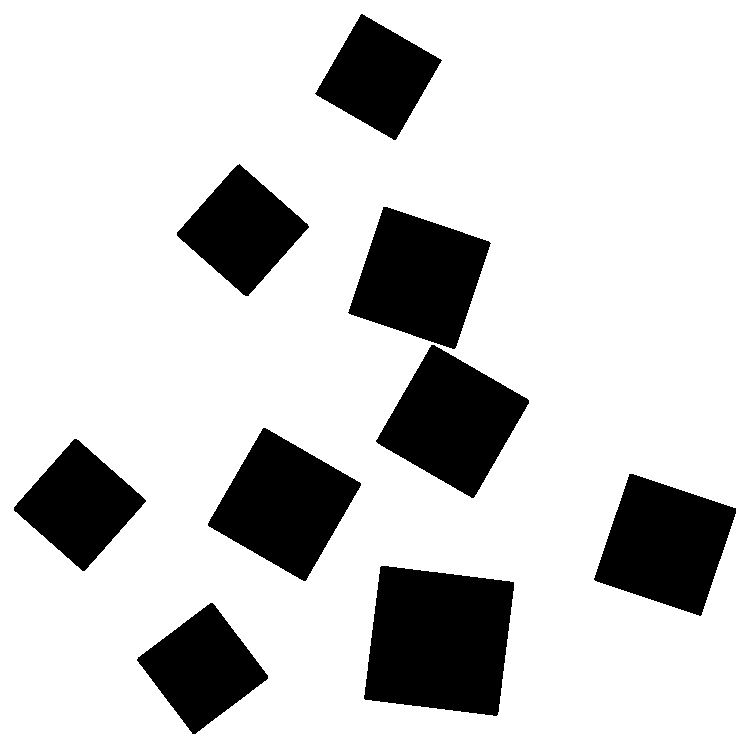
\includegraphics[scale=\s]{leaf2.pdf}
  \end{column}
  ...
    \begin{column}{3cm}
    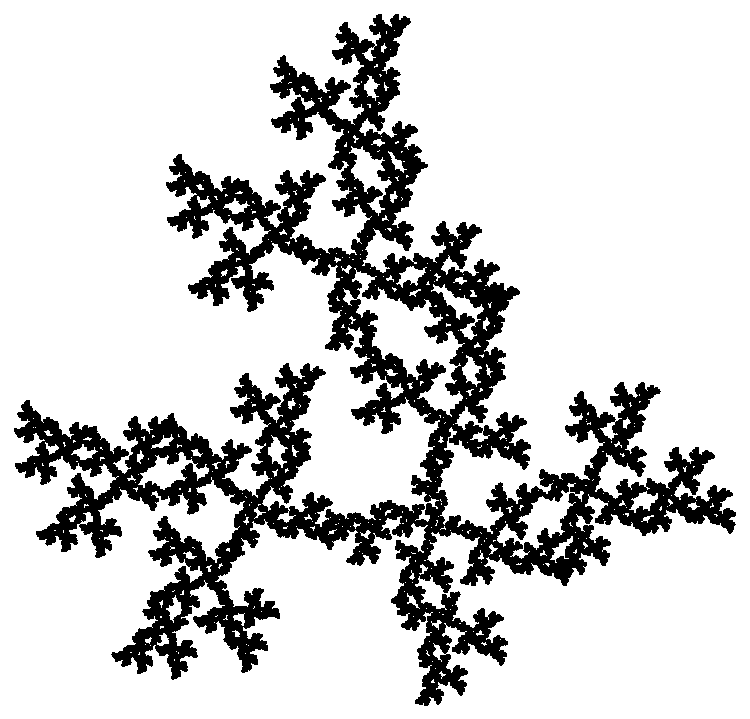
\includegraphics[scale=\s]{leafInfty.pdf}
  \end{column}
\end{columns}

\begin{itemize}
	\item Every fractal is approached by an IFS (Barnsley).
\end{itemize}

\end{frame}

\begin{frame}{Geometric construction}{``non-trivial'' fractals: Julia sets}
	\[ f_c(z) = z^2 + c \]
\begin{itemize}
	\item Define a recurrence $z_{n+1} = f_c(z_n)$
	\item Julia set: boundary of the convergence domain
\end{itemize}

\centering
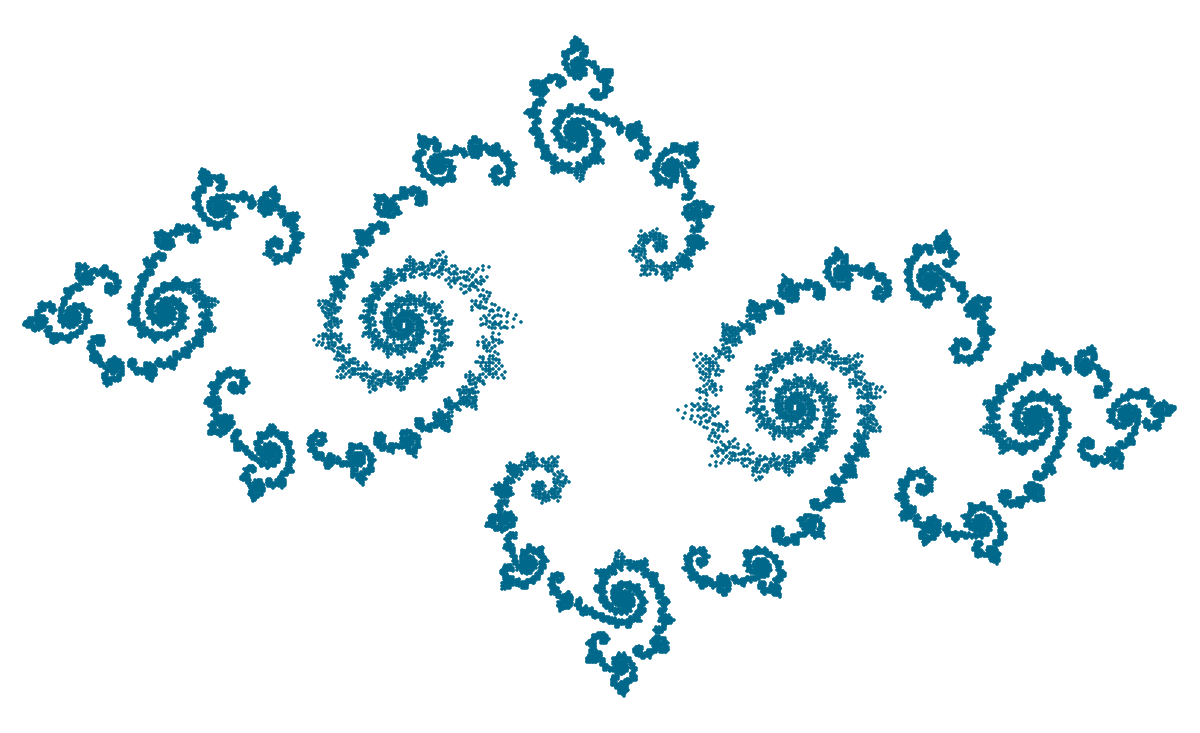
\includegraphics[scale=0.2]{julia.png}

\scriptsize
    Julia set $c = -0.77 + 0.22 i$

\end{frame}

\section{Derivation}
\subsection{Dummy}
\begin{frame}[allowframebreaks]{Time reversal polarization}
    \[ P^S = \frac{1}{2\pi} \int_{0}^{2\pi} \d k A^S(k) \]
	\begin{itemize}
        \item $s = I, II$ labelling Kramers partners
		\item Time reversal symmetry $\rightarrow$ \textit{half} the BZ is needed.\\
		\item Introduce the \textit{sewing matrix} $w_{\alpha \beta}(\vec{k}) \Ket{u_\beta(-\vec{k})} = \Theta\Ket{u_\alpha(\vec{k})}$
		\item Relate $P^I$ to the total polarization $P = P^I + P^{II}$
			\[ P^I = \frac{1}{2 \pi} \left( \int_0^\pi\d k A(k) + i \log \bigg[ \frac{\Pf[w(\pi)]}{\Pf[w(0)]} \bigg] \right) \]
	\end{itemize}
	
	\framebreak
	
	\[ P^I = \frac{1}{2 \pi} \left( \int_0^\pi\d k A(k) + i \log \bigg[ \frac{\Pf[w(\pi)]}{\Pf[w(0)]} \bigg] \right) \]
	
	\begin{itemize}
		\item Proof by explicit computation of the sewing matrix
		\[ 
		w(k) = 
		\begin{bmatrix}
		0 & - e^{-i \xi_{-k,\alpha}}\\
		e^{-i \xi_{k,\alpha}} & 0\\
		\end{bmatrix} \]
		in the $\Ket{u_\alpha^I(-k)} = e^{i \xi_{k,\alpha}} \Theta \Ket{u^{II}_\alpha(k)}$ representation.
		
		\item Gives indeed \[ \frac{i}{2 \pi} \log \bigg[ \frac{\Pf[w(\pi)]}{\Pf[w(0)]} \bigg] =  \sum_{\alpha} \xi_{\pi,\alpha} - \xi_{0,\alpha} = \frac{1}{2\pi}\int_{-\pi}^0\d{k} \left( A^I(k) - A^{II}(-k) \right) \]
	\end{itemize}
	
	\framebreak
	
	\begin{itemize}
		\item Time reversal polarization $P^T = P^I - P^{II}$
		\[ P^T = \frac{1}{2 \pi} \left( \int_0^\pi\d k \left[ A(k)-A(-k) \right] + 2 i \log \bigg[ \frac{\Pf[w(\pi)]}{\Pf[w(0)]} \bigg] \right) \]
		\item Using once again the sewing matrix 
		\[ A(-k) - A(k) = i \Tr\left[ w^\dagger(k) \nabla_k w(k) \right] = i \nabla_k \log \det \left[ w(k) \right] \]
		\item Final form
		\[  P^T = \frac{1}{i\pi} \log \left[ \frac{\sqrt{\det[w(\pi)]}}{\Pf[w(\pi)]} \frac{\Pf[w(0)]}{\sqrt{\det[w(0)]}} \right]  =  \frac{1}{i\pi} \log \left( \frac{\delta_{\pi}}{\delta_{0}} \right) \]
	\end{itemize}
\end{frame}

\section{Classification}
\subsection{Dummy}

\begin{frame}{Understand $\pi$}
 %   \includegraphics[width=\textwidth]{fu-kane-figure1.jpeg} \\
    \scriptsize
    taken from Fu, Kane, Mele 2007
\end{frame}

\begin{frame}{Relation between $\pi$ and $\delta$}
  %  \includegraphics[height=0.8\textheight]{fu-kane-figure2.jpeg}  \\
    \scriptsize
    taken from Fu, Kane, Mele 2007
\end{frame}


\begin{frame}{The $\mathbb{Z}_2$ invariants}
    \begin{align*}
        (-1)^{\nu_0} &= \prod_{n_j=0,1}{\delta_{n_1 n_2 n_3}} \\
        (-1)^{\nu_{i=1,2,3}} &= \prod_{n_{j\neq i}=0,1; n_i=1}{\delta_{n_1 n_2 n_3}}
    \end{align*}

$\Rightarrow \quad 4 \, \mathbb{Z}_2$ invariants \\
    $\Rightarrow \quad 2^4=16$ classes 
\end{frame}

    
\begin{frame}{$\mathbb{Z}_2$ invariants from TRIMs}
 %   \includegraphics[height=0.8\textheight]{fu-kane-figure2.jpeg} \\
    \scriptsize
    taken from Fu, Kane, Mele 2007

\end{frame}

\begin{frame}{weak and strong topological Insulators}
    \begin{itemize}
        \item weak: layers of 2D Quantum Spin Hall state
            \begin{itemize}
                \item $\nu_0$ = 0
                \item weak because 2 layers can combine to trivial insulator
            \end{itemize}
        \item strong: no layer picture, not built from 2D system
            \begin{itemize}
                \item $\nu_0$ = 1
            \end{itemize}
    \end{itemize}

    
\end{frame}

\section{Summary}
\subsection{Dummy}

\begin{frame}{Summary}

    \begin{itemize}
        \item 4 $\mathbb{Z}_2$ invariants $\Rightarrow$ 16 classes
        \item weak $\leftrightarrow$ strong
        \item general description of any crystaline surface by Miller indices
    \end{itemize}
\end{frame}

\begin{frame}{Outlook}
    Experimental realizations

    Materials
    \begin{itemize}
        \item Bi$_{x}$Sb$_{1 - x}$
        \item Bi$_2$Se$_3$
        \item Bi$_2$Te$_3$
        \item HgTe - under strain
    \end{itemize}
    
    
\end{frame}

\begin{frame}{References}

    \begin{itemize}
        \item Fu, Kane, Mele ``Topological Insulators in Three Dimensions'' (2007) PhysRevLett.98.106803
        \item Moore, Balents ``Topological invariants of time-reversal-invariant band structures'' (2007) PhysRevB.75.121306
        \item Bernevig, Hughes ``Topological Insulators and Topological Superconductors'' (2013) Princeton University Press
        \item Franz, Molenkamp ``Topological Insulators'' (2013) Springer
    \end{itemize}

\end{frame}

\end{document}
